% DO NOT COMPILE THIS FILE DIRECTLY!
% This is included by the other .tex files.

\begin{frame}[t,plain]
\titlepage
\end{frame}

\begin{frame}[t]{Topics for Today}
We will look at:

\begin{itemize}
\item Trans-dimensional MCMC
\item Nested Sampling
\end{itemize}

\end{frame}


\begin{frame}[t]{Trans-dimensional MCMC}
Trans-dimensional MCMC is useful when the model dimension is unknown.
\end{frame}

\begin{frame}[t]{Birth and Death}
For problems of unknown dimensionality, the hypothesis space is the union
of several fixed-dimension hypothesis spaces. Can add {\bf birth and death}
proposals that try to increase or decrease the number of objects in the model.

\begin{center}
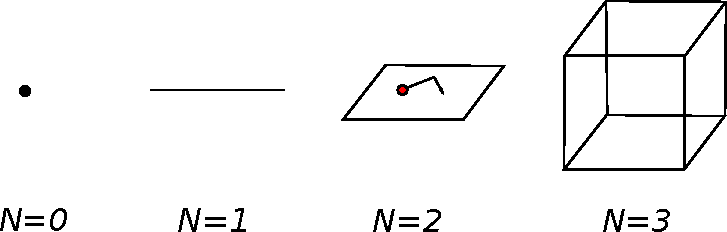
\includegraphics[scale=0.7]{drawing.pdf}
\end{center}

\end{frame}


\begin{frame}[t]{Challenging features}
\begin{center}
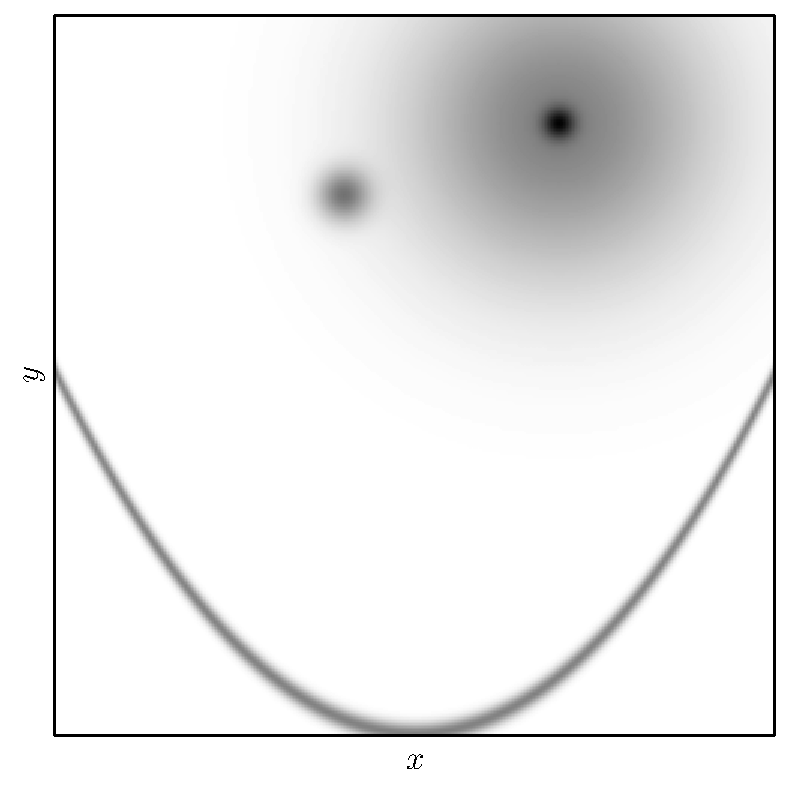
\includegraphics[scale=0.4]{challenges.pdf}
\end{center}
\end{frame}

\begin{frame}[t]{Nested Sampling}
In 2004, John Skilling introduced {\bf Nested Sampling}, a technique
that starts with the prior distribution, and shrinks volume at a controlled
rate. Maps big space into easy 1-D problem.

Resolves phase transition problem, and helps a little with multiple modes \&
strong degeneracies. Figure from Skilling (2006).

\begin{figure}
\begin{center}
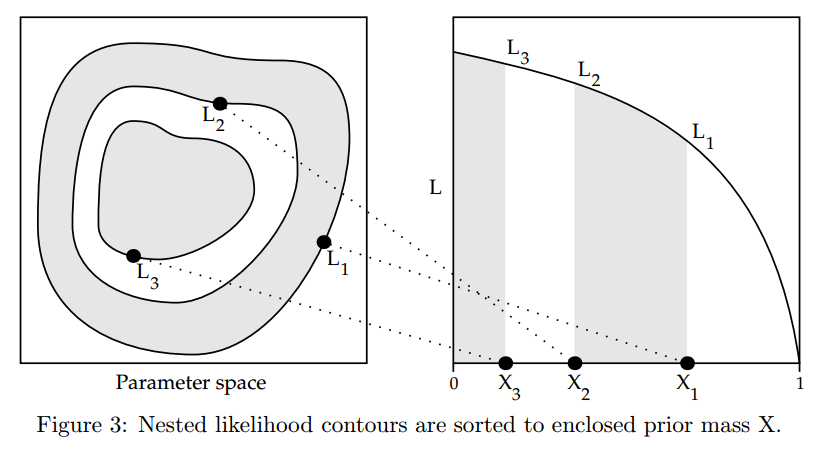
\includegraphics[scale=0.2]{ns.png}
\end{center}
\end{figure}

\end{frame}

